\documentclass[12pt,conference,a4paper,twocolumn]{IEEEtran}
\usepackage[left=2cm,right=2cm,top=2cm,bottom=2cm]{geometry}
\usepackage[utf8]{inputenc}
\usepackage[english]{babel}

\usepackage{amsmath}
\usepackage{amsfonts}
\usepackage{amssymb}
\usepackage{graphicx}
\usepackage{listings}
\usepackage{cite}
\usepackage{hyperref}
\hypersetup{colorlinks=false,linktoc=all,linkcolor=blue}
\usepackage{textcomp}
\usepackage{xcolor}
\usepackage{algorithmic}


\title{Control and Instrumentation Laboratory (EC692)\\Experiment No.: 1}
\author{	\IEEEauthorblockN{Dhiman Sarkar}
			\IEEEauthorblockA{\\
							Roll: 19101105086\\
							Dept. of Electronics and Comm. Engineering\\
							Jalpaiguri Government Engineering College\\
							Email: ds2286@ece.jgec.ac.in
							}
			\and
			\IEEEauthorblockN{Alok Barman}
			\IEEEauthorblockA{\\
							Roll: 19101105087\\
							Dept. of Electronics and Comm. Engineering\\
							Jalpaiguri Government Engineering College\\
							Email: ab2287@ece.jgec.ac.in
							}
			\and
			\IEEEauthorblockN{Alka Tigga}
			\IEEEauthorblockA{\\
							Roll: 19101105088\\
							Dept. of Electronics and Comm. Engineering\\
							Jalpaiguri Government Engineering College\\
							Email: at2288@ece.jgec.ac.in
							}
			\and
			\IEEEauthorblockN{Azizul Mallick}
			\IEEEauthorblockA{\\
							Roll: 19101105089\\
							Dept. of Electronics and Comm. Engineering\\
							Jalpaiguri Government Engineering College\\
							Email: am2289@ece.jgec.ac.in
							}
		}

\begin{document}
\maketitle
\begin{abstract}
	Familiarization with MATLAB control system toolbox and representation of pole zero and
transfer function of control system.
\end{abstract}

\section{Brief Description of The Experiment}
\begin{enumerate}
\item[a)] Defining a Polynomial to be used with Control-System-Toolbox.
\item[b)] Finding the roots of a polynomial.
\item[c)] Finding the Product of two polynomial.
\item[d)] Defining a Transfer Function.
\item[e)] Finding the Pole and Zero of a Transfer Function.
\item[f)] Generation Test Signals - Unit Step, Unit Ramp, Unit Impulse.
\end{enumerate}

\section{MATLAB Script}
\definecolor{mygrey}{gray}{0.97}
%\lstinputlisting{ec692_1.m}

\lstset{
  basicstyle=\tiny,
  columns=fullflexible,
  breaklines=true,
  postbreak=\mbox{{$\hookrightarrow$}\space},
  backgroundcolor=\color{mygrey},
  numbers=left,
  xleftmargin=3em,
  framexleftmargin=3em,
  %frame=single,
  %language=Matlab, 
  tabsize=3,
  escapeinside={\%latex}{\%latex},
}
\lstinputlisting[firstline=13,name=MATLAB]{ec692_1.m}



\section{Output Results and Plots}

\lstinputlisting[numbers=none]{ec692_1_console_out.txt}


\begin{figure}[t]
\centering
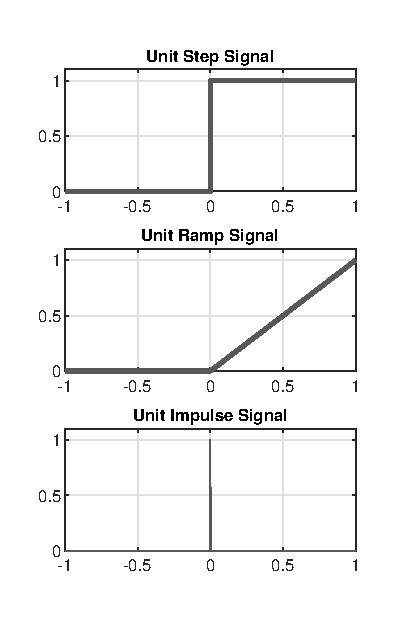
\includegraphics[width=3.5in]{ec692_1_plt.eps}
\caption{Generated Test Signals Output [see line number - \ref{s1},\ref{s2},\ref{s3}}
\label{signal}
\end{figure}

\begin{figure}[t]
\centering
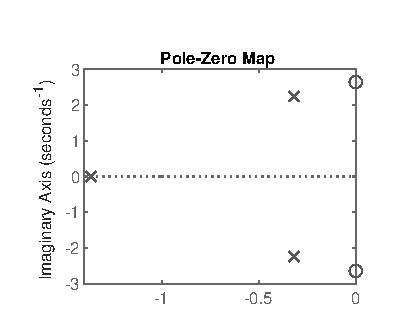
\includegraphics[width=3.5in]{ec692_2_plt.eps}
\caption{Pole-Zero Map of the transfer function \textit{tFcn} defined in line number.(\ref{tFcn}) of the MATLAB script.}
\label{pzplt}
\end{figure}

\section{Observations \& Conclusion}
We have already studied frequency domain analysis in \textit{Signals \& Systems} course. And now after being familiarized with MATLAB and MATLAB Control System Toolbox,\
we've learned to compute calculations in s-domain for more complex systems.

\section{Acknowledgment}
We would like to express our sincere gratitude to our course instructor Mr. Mirwaiz Rahaman and Mrs. Purba Basu for providing their invaluable guidance, comments and suggestions.

\end{document}